\Tsec{Билет №17}

\begin{leftrules}
Методы измерения констант нелинейного взаимодействия: метод z-сканирования.
\\ \phantom{42} \hfill \textit{лекция 8} 
\end{leftrules}

Метод измерения нелинейного показателя преломления, использующий эффект самофокусировки.

Измеряется зависимость энергии лазерного излучения, прошедшего через диафрагму, то есть коэффициент пропускания, в зависимости от положения образца относительно фокуса линзы. Затем из этой зависимости можно получить $n_2$ и $\Re \chi^{(3)}$.

Для измерения мнимой части $\chi^{(3)}$ диафрагму убирают и измеряют коэффиент поглощения.

\begin{figure}[ht]
    \centering
    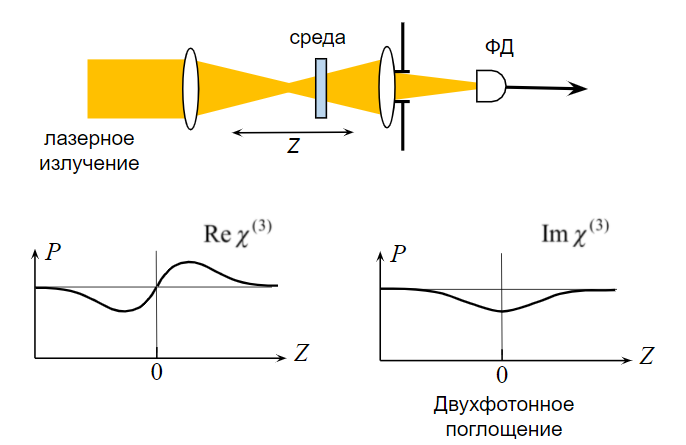
\includegraphics[width=0.5\textwidth]{figures/18_1.png}
    \caption{$z$-сканирование}
    %\label{fig:}
\end{figure}
